\chapter{評価}
\label{chap:evaluation}

本章では、ESP32マイコンとPC上で同一のWebAssemblyプログラムを実行することで、それぞれの環境における実行性能を比較し、マイコンにおけるWebAssembly実行環境の性能を考察する。

\section{評価手法}

\subsection{WebAssemblyバイナリ}
\label{subsec:wasm}

各実行環境で実行する同一のWebAssemblyプログラムとして、与えられた整数$n$に対して$n+1$番目のフィボナッチ数を返す関数$fib(n)$をC言語で実装した。

\begin{itembox}[l]{フィボナッチ関数のC言語による実装}
  \begin{verbatim}
    int fib(int n) {
      if (n <= 1) return 1;
      return fib(n - 1) + fib(n - 2);
    }
  \end{verbatim}
\end{itembox}

この関数のコンパイルには、LLVM/Clang 7.0.1を用いた。
LLVMのWebAssembly対応は試験的なものであるため、LLVMおよびClangコンパイラ自体を{\tt LLVM\_EXPERIMENTAL\_TARGETS\_TO\_BUILD}フラグに{\tt WebAssembly}を指定してソースコードからビルドした。

このLLVM/Clangを用いて{\tt fib}関数をコンパイルし、85バイトのWebAssemblyバイナリを得た。
コンパイル時に設定したオプションを表\ref{tab:compiler}に示す。

\begin{table}[htbp]
  \label{tab:compiler}
  \caption{ESP32環境の構成}
  \begin{center}
    \begin{tabular}{|l|l|}
    \hline
    --target=wasm32-unknown-unknown-wasm & wasm32バイナリを生成する \\ \hline
    -s & バイナリサイズを最適化(デバッグ情報などを含めない) \\ \hline
    -O3 & プログラムを最大レベルで最適化 \\ \hline
    -nostdlib -nostartfiles & 標準起動ファイルや標準ライブラリを用いない \\ \hline
    --fvisibility=default & 全ての関数をモジュール外から参照可能にする \\ \hline
    -Wl,--no-entry & エントリーポイント({\tt \_start})が無いことを警告しない \\ \hline
    \end{tabular}
  \end{center}
\end{table}

以下、全ての実行性能の比較にこのバイナリを用いた。

\subsection{ESP32環境}

\ref{subsec:wasm}項の方法によりコンパイルしたWebAssemblyバイナリを、\ref{chap:implementation}章で述べたESP32上のホストプログラムに埋め込み、libwasmを用いて0から30までの$n$について関数を呼び出した。

ESP32環境の構成を表\ref{tab:spec}に示す。

\begin{table}[htbp]
  \label{tab:spec}
  \caption{ESP32環境の構成}
  \begin{center}
    \begin{tabular}{|l|l|}
    \hline
    OS & ESP-IDF FreeRTOS v3.3-beta1-223-ga62cbfec9 \\ \hline
    ハードウェア & ESP32-WROOM-32 \\ \hline
    プロセッサ & Tensilica Xtensa LX6 (240MHz, dual-core) \\ \hline
    コンパイラ & GCC 5.2.0 (crosstool-NG 1.22.0-80-g6c4433a) \\ \hline
    \end{tabular}
  \end{center}
\end{table}

実行速度は、ESP-IDFが提供する\verb|esp_timer_get_time|関数を用いて計測した。
ESP-IDFを用いてコンパイルされたプログラムは、起動後\verb|esp_timer_init|関数を自動的に呼び出し、タイマーを初期化する。
\verb|esp_timer_get_time|関数は、このタイマーが初期化されてからの経過時間をマイクロ秒単位で返す。
0から13までの各$n$について、\verb|fib|関数の実行直前および実行直後に\verb|esp_timer_get_time|関数を呼び出し、差分を実行時間とした。

また、メモリフットプリントの計測には、FreeRTOSがAPIとして提供する \\
\verb|xPortGetMinimumEverFreeHeapSize|関数を用いた。
この関数は、起動以降一度も確保されていないヒープ領域の最小のサイズを返す。
すなわち、この値の減少分が、処理に必要なメモリフットプリントの増加分と言える。
そこで、モジュールのインスタンス化直後にこの関数で計測した値を0とし、フィボナッチ関数を実行した後の同関数が返す値との差分を取り、関数実行におけるメモリフットプリントとした。

\subsection{macOS環境}

ESP32環境と同様に、\ref{subsec:wasm}項の方法によりコンパイルしたWebAssemblyバイナリをmacOS上でlibwasmにより実行するプログラムを実装し、0から30までの$n$について関数を呼び出した。
macOS環境の構成を表\ref{tab:spec}に示す。

\begin{table}[htbp]
  \label{tab:spec}
  \caption{macOS環境の構成}
  \begin{center}
    \begin{tabular}{|l|l|}
    \hline
    OS & macOS 10.14.1 \\ \hline
    ハードウェア & Mac mini (2018) \\ \hline
    プロセッサ & Intel Core i5 (3 GHz, 6 cores) \\ \hline
    コンパイラ & Apple LLVM version 10.0.0 (clang-1000.11.45.5) \\ \hline
    \end{tabular}
  \end{center}
\end{table}

実行速度の計測には、OSが提供する\verb|clock_gettime|関数を用いた。
クロックの種別には \\
\verb|CLOCK_MONOTONIC|を指定し、時刻設定に関わらず単調増加する時間をナノ秒精度で取得した。

\subsection{ブラウザ環境}

macOS環境上で、libwasmとは別にWebブラウザによるWebAssembly実行性能も取得した。
JavaScriptスクリプト内でWebAssemblyバイナリを読み込み、同様に0から30までの$n$について関数を呼び出した。Webブラウザには、OS標準のSafari 12.0.1 (14606.2.104.1.1)を用いた。

また、実行時間の計測には、標準化されたWeb APIであるPerformance APIを用いた。
JavaScriptスクリプトから\verb|performance.now|関数を実行することで、仕様上はマイクロ秒の精度でタイムスタンプを得られる。
しかし、いわゆるSpectreと呼ばれる脆弱性への対策として、WebKitでは\verb|performance.now|の精度がミリ秒単位に丸められている\cite{webkit_spectre}\cite{webkit_trac}。
そこで、各$n$について\verb|fib(n)|を10000回ずつ実行し、その平均を実行時間の計測値として用いた。

\section{実行速度}

図\ref{tab:fib_time}に示す。

\begin{table}[htbp]
  \label{tab:fib_time}
  \caption{$n$ごとの{\tt fib}関数の実行時間と必要なクロック数の比(マイクロ秒)}
  \begin{center}
    \begin{tabular}{|r|r|r|r|}
      \hline
        & libwasm   & libwasm       &           \\ \hline
        & i5 3GHz   & ESP32 240MHz  & 必要クロック数の比 \\ \hline
      0  & 3         & 267           & 7  \\ \hline
      1  & 3         & 259           & 7  \\ \hline
      2  & 9         & 916           & 8  \\ \hline
      3  & 15        & 1,564         & 8  \\ \hline
      4  & 25        & 2,799         & 9  \\ \hline
      5  & 42        & 4,742         & 9  \\ \hline
      6  & 70        & 7,994         & 9  \\ \hline
      7  & 118       & 13,302        & 9  \\ \hline
      8  & 161       & 22,046        & 11 \\ \hline
      9  & 287       & 36,400        & 10 \\ \hline
      10 & 408       & 59,973        & 12 \\ \hline
      11 & 648       & 98,676        & 12 \\ \hline
      12 & 1,432     & 162,208       & 9  \\ \hline
      13 & 2,354     & 266,487       & 9  \\ \hline
      14 & 3,642     & 437,590       & 10 \\ \hline
      15 & 5,022     & 718,329       & 11 \\ \hline
      16 & 8,608     & 1,178,811     & 11 \\ \hline
      17 & 13,815    & 1,933,996     & 11 \\ \hline
      18 & 22,328    & 3,172,256     & 11 \\ \hline
      19 & 35,609    & 5,202,283     & 12 \\ \hline
      20 & 52,961    & 8,529,805     & 13 \\ \hline
      21 & 83,772    & 13,983,115    & 13 \\ \hline
      22 & 134,115   & 22,918,957    & 14 \\ \hline
      23 & 216,433   & 37,558,837    & 14 \\ \hline
      24 & 349,573   & 61,540,310    & 14 \\ \hline
      25 & 562,661   & 100,818,119   & 14 \\ \hline
      26 & 909,827   & 165,139,586   & 15 \\ \hline
      27 & 1,455,711 & 270,457,743   & 15 \\ \hline
      28 & 2,353,144 & 442,878,521   & 15 \\ \hline
      29 & 3,847,535 & 725,117,084   & 15 \\ \hline
      30 & 6,237,998 & 1,187,057,130 & 15 \\ \hline
    \end{tabular}
  \end{center}
\end{table}

\section{メモリフットプリント}

また、同プログラムについて、メモリフットプリントとしてヒープ領域に確保されるメモリの最大量を計測した。

FreeRTOSがAPIとして提供する\verb|xPortGetMinimumEverFreeHeapSize|関数は、起動以降一度も確保されていないヒープ領域の最小のサイズを返す。
すなわち、この値の減少分が、処理に必要なメモリフットプリントの増加分と言える。
そこで、モジュールのインスタンス化直後にこの関数で計測した値を0とし、フィボナッチ関数を実行した後の同関数が返す値との差分を取り、関数実行におけるメモリフットプリントとした。

引数\verb|n|を0から13まで変化させた際の、関数実行のメモリフットプリントの推移を図\ref{fig:heap_size}に示す。

\begin{figure}[htbp]
  \caption{メモリフットプリントの推移とその比較}
  \label{fig:heap_size}
  \begin{center}
    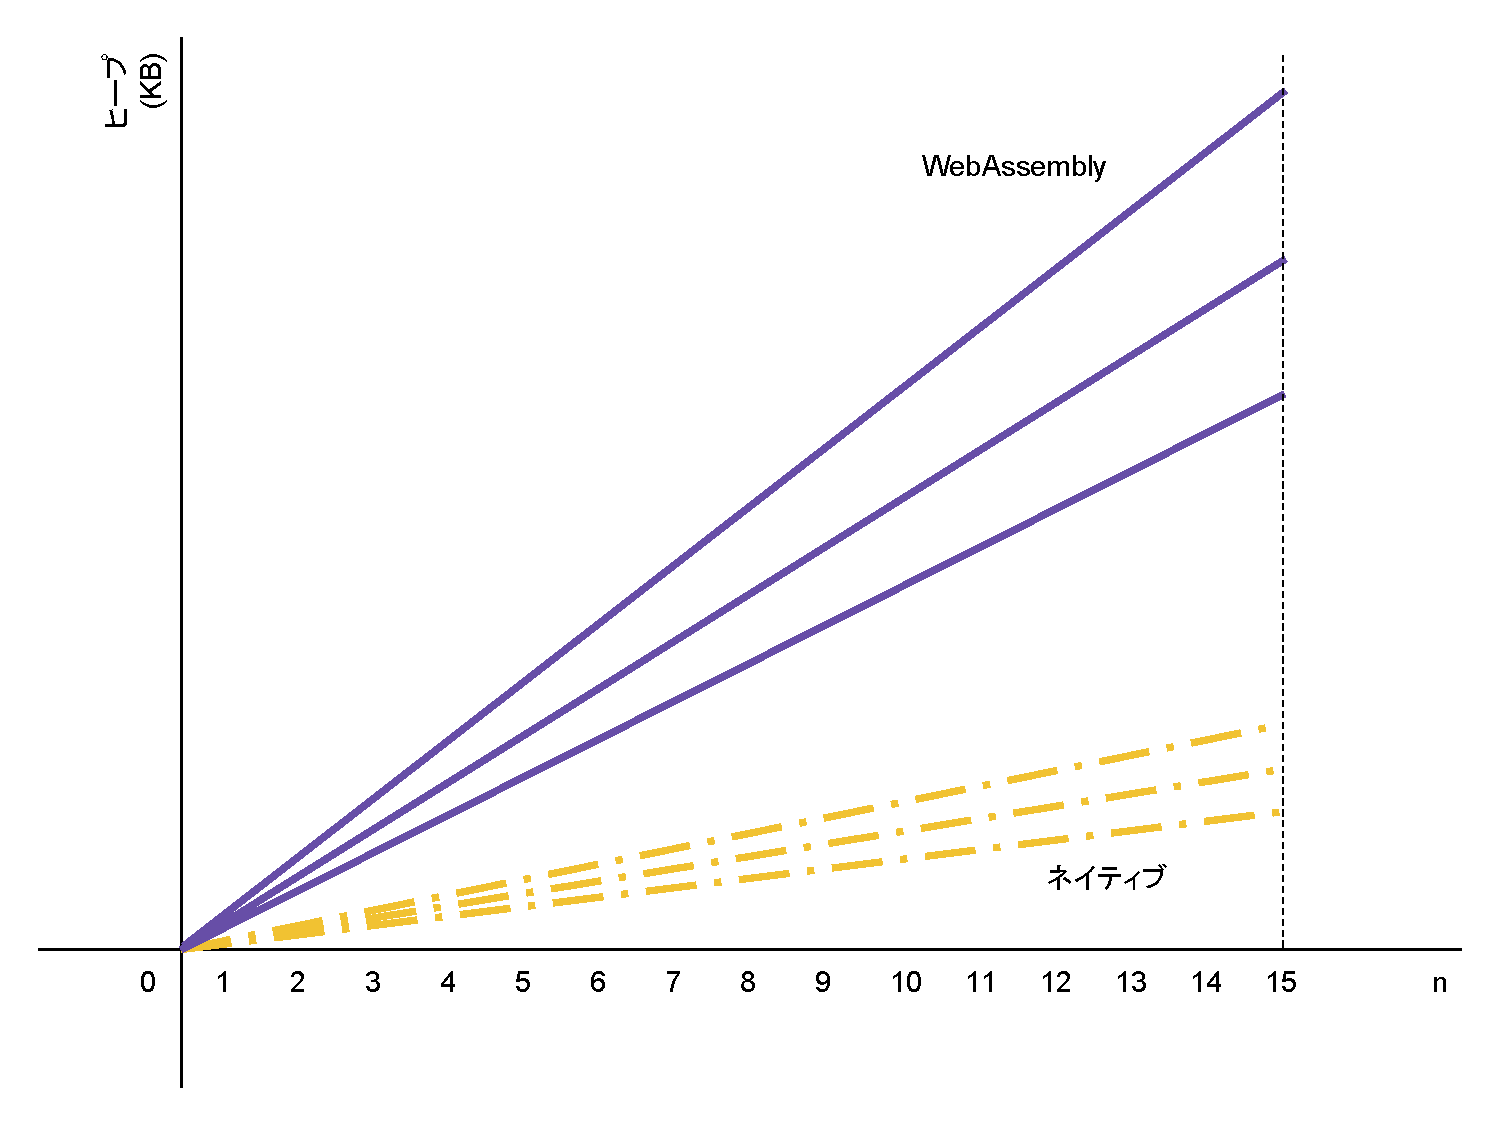
\includegraphics[bb=0 0 600 370,width=10cm]{img/heap_size.pdf}
  \end{center}
\end{figure}

定数を返すのみである$n=0$および$n=1$の時、メモリフットプリントは540バイトで、実行速度と同様に変化はなかった。
再帰的な関数呼び出しが発生する$n=2$以降は、208バイトずつ上昇していった。
これは、WebAssembly実行環境のスタックにおけるメモリ消費であると考えられる。

